\chapter{Evaluation} \label{chap:evaluation}

The aim of this Chapter is to present the experimental evaluation of our system.
Firstly, in \S\ref{sec:evaluation:hardware} we introduce the hardware used for the benchmarking.
We differentiate between the machines and software used in the Server-side \S\ref{sec:evaluation:hardware:server} and those used in the Client-side \S\ref{sec:evaluation:hardware:client} since both components have very different requirements.
%For instance, server machines must have \sgx available and enclaves enabled.
Secondly, we cover the different experimental configurations considered in \S\ref{sec:evaluation:experiments}.
The latter require a given number of metrics that we present in \S\ref{sec:evaluation:metrics}.
The workloads used to assess the performance are presented and justified in \S\ref{sec:evaluation:workload}.
Lastly, our results are presented and analyzed in \S\ref{sec:evaluation:results}.
In a nutshell, our experiments answer the following questions: \emph{(i)} is the design of the platform sound? \emph{(ii)} is our implementation efficient, \emph{(iii)} what is the overhead of SGX, and \emph{(iv)} is it scalable?

\section{Hardware Settings} \label{sec:evaluation:hardware}

\subsection{Server} \label{sec:evaluation:hardware:server}
The server side is where the filesystem interface is hosted and where the \textsc{SGX-Spark} jobs run.
Therefore, it must be be equipped with \textsc{Intel SGX} and enclave mode must be enabled. 
The component runs on a machine located at the University of Neuch\^atel's (UniNe) cluster with Intel~\textregistered\xspace Xeon~\textregistered\xspace CPU E3-1270 v6 @ $3.80$~GHz with 8 cores and 64 GiB RAM. 
We use Ubuntu $16.04$ LTS (kernel 4.19.0-41900-generic) and the official Intel~\textregistered\xspace SGX driver v$2.0$~\cite{sgx-driver}, and \textsc{SGX-LKL}~\cite{sgx-lkl}. 
We use an internal release of the \textsc{SGX-Spark} framework, which is currently under development.

\subsection{Client} \label{sec:evaluation:hardware:client}
For evaluation purposes, and as introduced in the Implementation Chapter (\ref{chap:implementation}), the whole set of clients is deployed as a standalone Docker swarm in a single computing instance. 
The machine we are using is located in UniNe's cluster and is equipped with two AMD EPYC 7281 16-Core Processor which, taking hyperthreading into consideration, account for a total of 64 cores and 64 GiB RAM. 
It is deployed with Ubuntu v$18.04$ LTS (kernel 4.15.0-42-generic). 
The client containers are built and deployed using Docker (v$18.09.0$) and \texttt{docker-compose} (v$1.23.2$). 
We use \texttt{docker-machine} (v$0.16.0$) with the \texttt{virtualbox} disk image. 
Each machine hosts 20 clients, the maximum number of services supported by its local network, and it registers itself to the Swarm via a name discovery service running on another machine (we rely on \textsc{Consul}~\cite{consul-image}).
Inter-container communication is established using the \texttt{overlay} network driver.
To optimize start up time we provide all the images via \texttt{.tar} files that are loaded to the VM, skipping image building time, and we use a local copy of \texttt{virtualbox}'s disk image.
In order to gather the results, we mount a Docker volume on each client and mirror the VM to the real filesystem using \textit{Secure SHell File System (SSHFS)}. 
We pull the latest images available on Docker Hub for the Consul name discovery service (v$1.4$) and the \texttt{eclipse-mosquitto} (v$1.5$) message broker.

\section{Experimental Configuration} \label{sec:evaluation:experiments}

In order to evaluate the overhead \sgxspark and our system introduce, we compare three different settings or execution modes:
\begin{enumerate}
    \item The \textbf{vanilla Spark} mode acts as our baseline. It executes the algorithm using a standard distribution of the Spark cluster-computing framework.
    \item The \textbf{\sgxspark w/o Enclaves} mode is an \sgxspark execution but with the enclaves disabled. This is, the engine sets up the collaborative JVM scheme communicating over SHM, but neither runs inside an enclave.
    \item The \textbf{\sgxspark w/ Enclaves} mode is the execution mode of our system. It runs unmodified Spark applications leveraging \sgx for sensitive computations.
\end{enumerate}
The current implementation of \sgxspark (still under development) does not provide support for Spark's \texttt{Streaming Context} inside enclaves. 
To overcome this temporary limitation, we evaluate the \texttt{SDNN} and \texttt{Identity} algorithms in \emph{batch} and \emph{stream} mode. 
For the former, all three different execution modes are supported.
For the latter, we present estimated results for \sgxspark with enclaves enabled, basing the computation time on the batch execution times and the additional overhead against the other modes.

The algorithms are fed with a data file or a data stream, respectively.
We increment the input workload (see \S\ref{sec:evaluation:workload}) and measure the impact it has on the execution time (see \S\ref{sec:evaluation:metrics}).
In batch mode, a result file is generated once the processing is finished.
In the streaming scenario, an output file is generated every ten seconds.
In a multi-client scenario, each client has a separated data stream (or file) and consequently a different result file.
A streaming execution consists of 5 minutes of the service operating with a specific execution mode, client configuration, and input workload.
We execute our experiments 5 times and report average values together with their standard deviations.

\section{Analyzed Metrics} \label{sec:evaluation:metrics}

To assess performance, scalability, and efficiency, we consider two different metrics depending on whether we run in \emph{batch} or \emph{stream} mode: \textbf{elapsed time} and \textbf{average batch processing time}
\footnote{
Note that we mention \textit{batch} in two different contexts: batch execution (one static input and static output) and streaming batches.
Spark Streaming divides live input data in chunks called \emph{batches} determined by a time duration (10 seconds in our experiments).
The time it takes the engine to process the data therein contained is denoted as batch processing time.}.
\begin{enumerate}
    \item \textbf{Elapsed Time} measures the time it takes the engine to process the input file. In short, it is our system's execution time in \emph{batch} mode. To obtain this metric it is sufficient with introducing logs (measuring time) in the application code.
    \item \textbf{Average Batch Processing Time} takes the average of the time it takes the platform to process each 10-second-long chunk of the input data stream. To obtain this value we query Spark's REST API~\cite{spark-rest-api}. We use Python's \texttt{requests} package as depicted in Listing~\ref{code:evaluation:requests}. Since the server, the clients, and the deployment might be hosted in different locations, the easiest way to query the REST API instantiated by the master process at the server is to establish a SSH tunnel and forward the contents in the server's $4040$ port to \texttt{localhost}. This is done in line 9 using an additional Python script that we attach in Listing~\ref{code:evaluation:port-forward} (see also Listing~\ref{code:evaluation:forward-tunnel}). Note that in the latter there are configuration-specific parameters. Once the port forwarding is established, we set up and execute the request (lines 11-14) and then process the results (lines 16-20). It is worth mentioning that, since Spark keeps an historic of the batch processing times, it is sufficient with doing only one query right before we terminate the 5-minute-long execution.
\begin{lstlisting}[language=Python,caption={Snippet illustrating a query to Spark's REST API.},label=code:evaluation:requests]
def query_batch_processing(filedir):
    """Query Spark's REST API 

    This method queries sparks API for the batch processing time. It firsts
    launches a port forwarding daemon in order to be able to perform the
    request and then queries the information. Note that this is done only
    once at the end of the execution (right before killing it).
    """
    proc = subprocess.Popen("python3 port_forward.py".split(" "))
    time.sleep(2)
    app_id = requests.get('http://localhost:4040/api/v1/applications/').json()
    app_id = app_id[0]['id']
    req = 'http://localhost:4040/api/v1/applications/{}/jobs/'.format(app_id)
    r = requests.get(req).json()
    time_format = "%Y-%m-%dT%H:%M:%S.%f"
    times = [ datetime.strptime(r[i]['completionTime'][:-3],
                                time_format).timestamp() -
              datetime.strptime(r[i]['submissionTime'][:-3],
                                time_format).timestamp()
              for i in reversed(range(len(r))) if 'completionTime' in r[i] ]
    proc.kill()
    filename = filedir + "batch_processing_times.csv"
    with open(filename, "w+") as f:
        for num, val in enumerate(times):
            if num == 0:
                f.write("{} {}".format(num, val))
            else:
                f.write("\n{} {}".format(num, val))
    return 0
\end{lstlisting}
\end{enumerate}
We study the variability of these two parameters as we modify the input workload according to \S\ref{sec:evaluation:workload}.

\vspace{-20pt}

\section{Workload} \label{sec:evaluation:workload}

As firstly introduced in Chapter \S\ref{sec:background:med}, the clients inject streams as cardiac signals corresponding to RR intervals and their timestamps.
Each client injects a modest workload into our system (230 - 690 bytes per minute).
\begin{table}[h!]
    \centering
    \caption[Different input loads used for Batch Mode (BM) and Stream Mode (SE)]{Different input loads used for Batch Mode (BM) and Streaming Mode (SM). We present the sample rate they simulate (\textit{i.e.} how many RR intervals are streamed per second) and the overall file or stream size (Input Load). \label{tab:eval:inputs}}
    \vspace{6pt}
    \begin{tabular}{L{3.5cm}C{7.0cm}C{5.5cm}}
        \toprule
        \textbf{Experiment} & \textbf{\texttt{s\_rate} (samples / sec)} & \textbf{Input Load}\\[1pt] \midrule 
        BM - Small Load & $\lbrace 44, 89, 178, 356, 712, 1424 \rbrace $ & $\lbrace 1, 2, 4, 8, 16, 32 \rbrace$ kB \\[1pt] 
        SM - Small Load & $\lbrace 44, 89, 178, 356, 712, 1424 \rbrace$ & $\lbrace 1, 2, 4, 8, 16, 32 \rbrace$ kB / sec\\[1pt] 
        BM - Big Load & $\lbrace 44, 89, 178, 356, 712, 1424 \rbrace * 1024$ & $\lbrace 1, 2, 4, 8, 16, 32 \rbrace$ MB \\[1pt] 
        SM - Big Load & $\lbrace 44, 89, 178, 356, 712, 1424 \rbrace * 1024$ & $\lbrace 1, 2, 4, 8, 16, 32 \rbrace$ MB / sec\\[1pt] 
        \bottomrule
    \end{tabular}
\end{table}
Hence, to assess the efficiency and the processing time as well as to uncover possible bottlenecks, we scale up the output rate of these signals with the goal of inducing more aggressive workloads into the system.
We do so in detriment of medical realism, since arbitrary input workloads do not relate to any medical situation or condition.
Table~\ref{tab:eval:inputs} shows the variations used to evaluate the various execution modes.
On the leftmost column, BM and SM stand for \emph{batch} and \emph{stream} mode execution. For each mode, we consider a small load and a big load evaluation setting. We present both the \texttt{sample\_rate} parameter passed to the \texttt{sensor} component and the total workload that amounts to (in multiples of bytes per second).

\vspace{-7pt}

\section{Results} \label{sec:evaluation:results}

\vspace{-11pt}

In this Section we present and analyze the evolution of the different metrics (\S\ref{sec:evaluation:metrics}) as we vary the input workload (\S\ref{sec:evaluation:workload}) for the different execution modes (\S\ref{sec:evaluation:experiments}).
We firstly present the results for \emph{batch} mode in \S\ref{sec:evaluation:results:batch} and then we do the same for \emph{stream} mode in \S\ref{sec:evaluation:results:stream}.

\vspace{-19pt}

\subsection{Batch Execution} \label{sec:evaluation:results:batch}

\vspace{-8pt}

The exact configuration for the study of the elapsed time as we vary the input file size is: one client, one master, one driver, one worker, and a variable input file that progressively increases in size. 
We measure the elapsed time of each execution and present the average and standard deviation of a total of five experiments with the same configuration.
Results obtained are included in Figure \ref{fig:batch-input-size}.

\begin{figure}[h!]
    \centering
    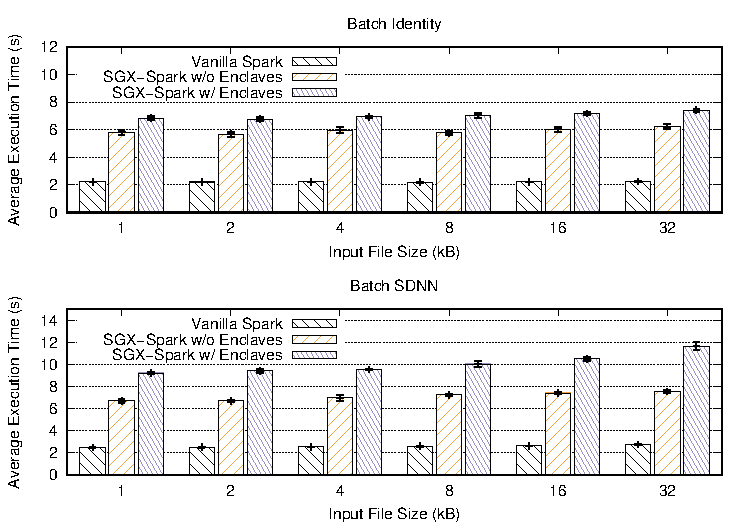
\includegraphics[width=.85\textwidth]{plots/batch/input_size/input_size.pdf}
    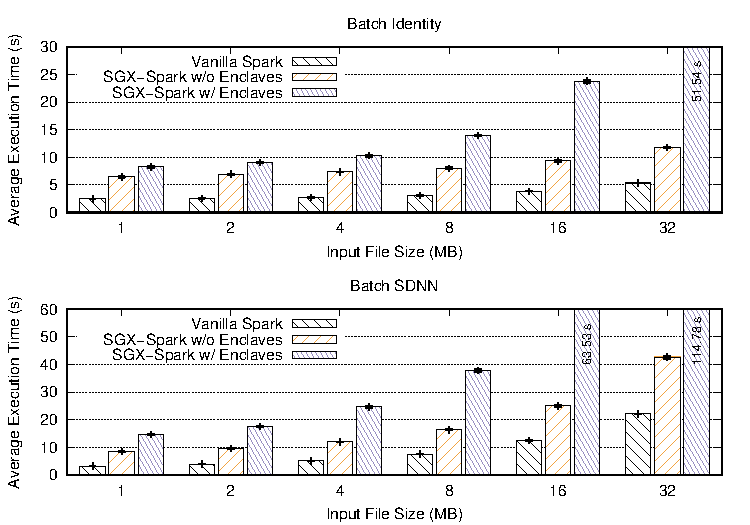
\includegraphics[width=.85\textwidth]{plots/batch/input_size/big_input_size.pdf}
    \caption[Evolution of the average elapsed (execution) time as the input workload increases.]{Evolution of the average elapsed time, together with its standard deviation, as we increase the size of the input file. We compare the three different execution modes for each algorithm. Mode \sgxspark w/ enclaves is the mode the platform runs in. \label{fig:batch-input-size}}
\end{figure}

From the bar plot we highlight that the variance between execution times among same execution modes as we increase the input file size is relatively low. 
However, it exponentiates as we reach input files of 4-8 MB.
We also observe that the slow-down factor between execution modes remains also quite static until reaching the before mentioned load threshold. 
\sgxspark with enclaves (and hence our system), if input files are smaller than 4 MB, increases execution times x4-5 when compared to vanilla Spark and x1.5-2 when compared to \sgxspark with enclaves disabled.
Note that, since a single client in our real use case streams around 230 to 690 bytes per minute, the current input size limitation already enables several hundreds of concurrent clients (considering processing time as the only bottleneck).

\vspace{-19pt}

\subsection{Stream Execution} \label{sec:evaluation:results:stream}

\vspace{-8pt}

Similarly as done in \S\ref{sec:evaluation:results:batch}, we scale the load of the data streams that feed the platform and study the evolution of the average batch processing time.
We deploy one worker, one driver and one client, query the average batch processing time to Spark's REST API, and present the results for the \texttt{Identity} and \texttt{SDNN} algorithms. 
Results are summarized in Figure \ref{fig:throughput}.

\begin{figure}[h!]
    \centering
    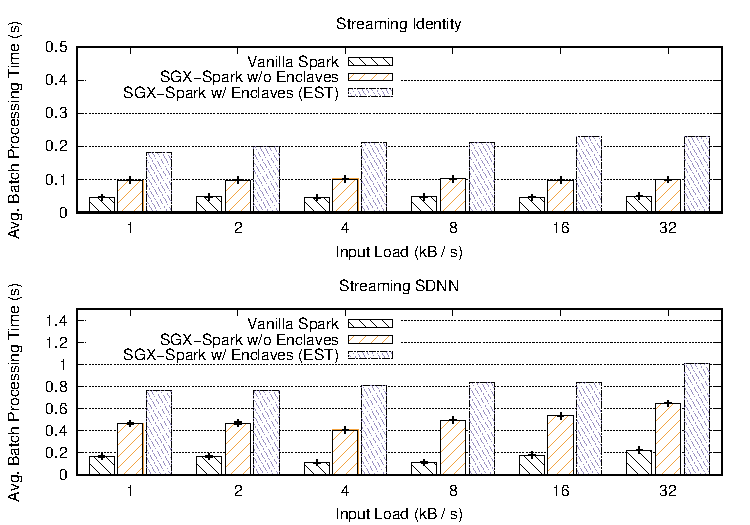
\includegraphics[width=.85\textwidth]{plots/stream/input_size/throughput.pdf}
    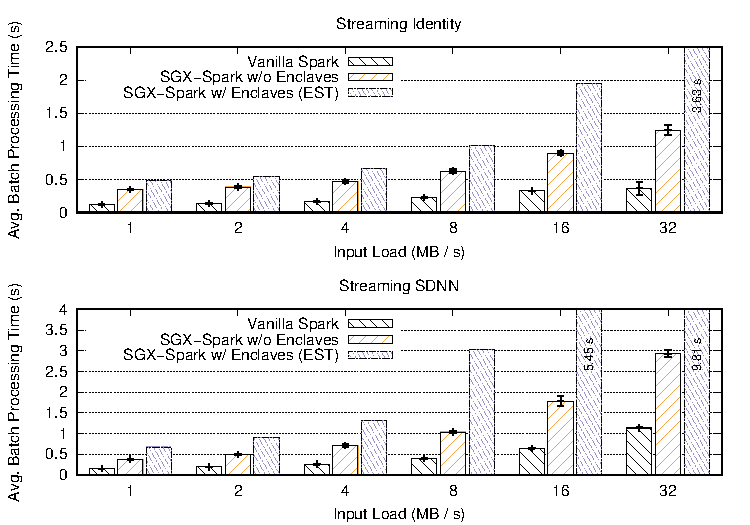
\includegraphics[width=.85\textwidth]{plots/stream/input_size/big_throughput.pdf}
    \caption[Evolution of the average batch processing time as we increase the input stream size.]{Evolution of the average batch processing time as we increase the input stream size. We compare the results of the three different execution modes. Note that those corresponding to \sgxspark w/ enclaves are estimated basing on the results in Figure \ref{fig:batch-input-size} and the slow-down with respect to the other execution modes. \label{fig:throughput}}
\end{figure}

We obtain results for vanilla Spark, and \sgxspark without enclaves, and we estimate them for \sgxspark with enclaves.
We observe similar behaviours as those in Figure \ref{fig:batch-input-size}. 
Variability among same execution modes when increasing the input stream size is low until reaching values of around 4 to 8 MB per second.
Similarly, the slow-down factor from vanilla Spark to \sgxspark without enclaves remains steady at around x2-2.5 until reaching the load threshold.
As a consequence, it is reasonable to estimate that the behaviour of \sgxspark with enclaves will preserve a similar slow-down factor ($\times$4-$\times$5) when compared with vanilla Spark in streaming jobs.
Similarly, the execution time will increase linearly with the input load after crossing the load threshold of 4 MB.
Note as well how different average batch processing times are in comparison with elapsed times, in spite of relatively behaving similar. 
This is due to the fact that the average of streaming batch processing times smoothens the initial overhead of starting the Spark engine. 
Furthermore, in \emph{stream} mode, data loading times are hidden under previous batches' execution times, and, again, smoothened by the average.
